\chapter{Experiments}

In this chapter we discuss the experiments we conducted to compare the performance of \ac{LVNMT} models with and without normalizing flows, as well as other experiments to empirically evaluate the impact of latent variables \ac{NMT} system.  

Our hyper-parameters for the models used in this thesis predominantly follow the values in \cite{eikema2018AEVNMT}. We include explicit values specific to our implementations in the supplement material. Generally speaking, all our \ac{GRU} consist of a single 256 hidden unit layer for each component, and our word embeddings are 256 units.

To help prevent \textit{posterior collapse} in which the latent variable is ignored during training, we apply KL annealing and word dropout. KL annealing involves annealing the KL divergence term in the \ac{ELBO} during training \cite{bowman2015GeneratingSent}. We anneal  linearly over the first 80,000 steps. Word-dropout involves replace word embeddings with the unknown embedding with some $p$ probability to encourage the model to rely more on the latent variable. We choose a dropout rate of 0.1 for both models, although previous work suggested that this word dropout didn't necessarily help in the discriminative \ac{NMT} case \cite{harshil2018GNMT}. \reminder{depending on performance of VNMT might move to doing the pretrained trick they describe}

We conducted our experiments with the IWSLT 2016 data sets available in the torch text library. \footnote{https://github.com/pytorch/text} We chose to use the De-En, Ar-Enlanguage pairs as these are languages we could more naturally evaluate subjectively, although we explicitly note we did not do any formal human evaluation of translation quality. We list total sentence counts in the supplement material, and note that the counts vary between certain symmetrical language directions as these were the splits provided by the Torch Text library. \reminder{move last bit to supplement material, when you do add it also note that with the current TorchText we had to manually combine data as they do not do so with the current implementation}

We represented our vocabulary for each language with \ac{BPE} \cite{sennrich2015NMTRarwordsBPE}. We used a vocabularly of 10,000 \ac{BPE}s per language, because we found that larger vocabularies resulted in sub-word units that occurred infrequently enough to be uninformative from a practical learning perspective. We performed \ac{BPE} using the Sentence Piece library. \footnote{https://github.com/google/sentencepiece} We trained our \ac{NMT} models on sequences of maximum length 50. The only other normalizing we did on our data sets was removing diacritics from the Arabic sentences. 

Although most research in \ac{NMT} literature use beam search decoding, we choose to to use greedy decoding when translating sentences. Our general assumption is that if normalizing flows help with translation, this would carry over to heuristic searchers like beam search. Also, in recent literature studying the impact of beam search, larger beams do not necessarily translate to providing huge improvements in performance \cite{cohen2019unconstrained}. \reminder{ this...is a cop out midly because I saw performance degredation with my beam search algorithm set to 10... it worked fine on a 4,000,000 mil sentence dataset but that took waaaay to long}

- Our networks use hidden layer sizes and embeddings of size 256 which is similar to the choices made in [eikeman et. al 2018] and we found for VNMT these parameters also worked better than those in [vnmt et. al.] for preliminary experiments on the WMT 2014 data they evaluated on. All specific params are in supplement material.
We limit ourselves to these datasets, because it allows us to consider multiple language pairs and is a manageable size for our available computation budget. Due to these constraints, we caution readers that our results may not be applicable to datasets of different sizes.

\section{General Translation}

In this section we report our experimental results including normalizing flows in existing \ac{LVNMT} systems. Our hypothesis was that, given normalizing flows success in computer vision, that similar gains can be achieved by including normalizing flows on top of previously considered \ac{LVNMT} systems.  

Our baselines include the \ac{LVNMT} models we described in Chapter 2 without normalizing flows whose posterior distribution is the Isotropic Gaussian. To provide more fair comparison, our baselines optimized the \ac{ELBO} with the same number of Monte Carlo samples as our normalizing flows models. In these baseline cases, this corresponds to better approximations of the negative log-likelihood of sequence predictions. The KL divergence is analytic in the Gaussian case which does not require sampling \cite{kingma2014autoencodingVB,rezende2014stochasticBackprop}.

 Table \ref{tab:de_en_besttranslations} shows the BLEU score of our results on the test set after choosing the best performing models based on the validation set. 

\begin{table}[] 

	\caption{BLEU score for our models with an increasing number of normalizing flows for De - En translation. The best performing models are in bold for each type of flow. }
	\label{tab:de_en_besttranslations}
\begin{tabular}{llllllll}
	\multicolumn{8}{c}{\textbf{Latent Dimension: 2}}                                                                                                                                                                                                                                                                                                                                                                                                                                                                                                         \\ \hline
	\multicolumn{1}{|l|}{\textbf{Flows}}                          & \multicolumn{1}{l|}{\textbf{1}}                              & \multicolumn{1}{l|}{\textbf{2}}                              & \multicolumn{1}{l|}{\textbf{4}}                              & \multicolumn{1}{l|}{\textbf{8}}                              & \multicolumn{1}{l|}{\textbf{16}}                             & \multicolumn{1}{l|}{\textbf{Baseline}}                                         & \multicolumn{1}{c|}{\textbf{Model}}                                          \\ \hline
	\rowcolor[HTML]{F9F9E1} 
	\multicolumn{1}{|l|}{\cellcolor[HTML]{F9F9E1}Planar}          & \multicolumn{1}{l|}{\cellcolor[HTML]{F9F9E1}\textbf{19.062}} & \multicolumn{1}{l|}{\cellcolor[HTML]{F9F9E1}18.949}          & \multicolumn{1}{l|}{\cellcolor[HTML]{F9F9E1}18.935}          & \multicolumn{1}{l|}{\cellcolor[HTML]{F9F9E1}19.009}          & \multicolumn{1}{l|}{\cellcolor[HTML]{F9F9E1}19.051}          & \multicolumn{1}{l|}{\cellcolor[HTML]{F9F9E1}}                                  & \multicolumn{1}{l|}{\cellcolor[HTML]{F9F9E1}}                                \\ \cline{1-6}
	\rowcolor[HTML]{F9F9E1} 
	\multicolumn{1}{|l|}{\cellcolor[HTML]{F9F9E1}IAF}             & \multicolumn{1}{l|}{\cellcolor[HTML]{F9F9E1}18.894}          & \multicolumn{1}{l|}{\cellcolor[HTML]{F9F9E1}18.477}          & \multicolumn{1}{l|}{\cellcolor[HTML]{F9F9E1}18.803}          & \multicolumn{1}{l|}{\cellcolor[HTML]{F9F9E1}\textbf{18.964}} & \multicolumn{1}{l|}{\cellcolor[HTML]{F9F9E1}18.67}           & \multicolumn{1}{l|}{\multirow{-2}{*}{\cellcolor[HTML]{F9F9E1}18.924}}          & \multicolumn{1}{l|}{\multirow{-2}{*}{\cellcolor[HTML]{F9F9E1}VNMT}}          \\ \hline
	\rowcolor[HTML]{F4DAD8} 
	\multicolumn{1}{|l|}{\cellcolor[HTML]{F4DAD8}Planar}          & \multicolumn{1}{l|}{\cellcolor[HTML]{F4DAD8}20.773}          & \multicolumn{1}{l|}{\cellcolor[HTML]{F4DAD8}20.696}          & \multicolumn{1}{l|}{\cellcolor[HTML]{F4DAD8}20.808}          & \multicolumn{1}{l|}{\cellcolor[HTML]{F4DAD8}20.863}          & \multicolumn{1}{l|}{\cellcolor[HTML]{F4DAD8}19.33}           & \multicolumn{1}{l|}{\cellcolor[HTML]{F4DAD8}}                                  & \multicolumn{1}{l|}{\cellcolor[HTML]{F4DAD8}}                                \\ \cline{1-6}
	\rowcolor[HTML]{F4DAD8} 
	\multicolumn{1}{|l|}{\cellcolor[HTML]{F4DAD8}IAF}             & \multicolumn{1}{l|}{\cellcolor[HTML]{F4DAD8}20.607}          & \multicolumn{1}{l|}{\cellcolor[HTML]{F4DAD8}20.515}          & \multicolumn{1}{l|}{\cellcolor[HTML]{F4DAD8}20.582}          & \multicolumn{1}{l|}{\cellcolor[HTML]{F4DAD8}20.552}          & \multicolumn{1}{l|}{\cellcolor[HTML]{F4DAD8}20.464}          & \multicolumn{1}{l|}{\multirow{-2}{*}{\cellcolor[HTML]{F4DAD8}\textbf{21.024}}} & \multicolumn{1}{l|}{\multirow{-2}{*}{\cellcolor[HTML]{F4DAD8}GNMT}}          \\ \hline
	\multicolumn{8}{c}{\textbf{Latent Dimension: 128}}                                                                                                                                                                                                                                                                                                                                                                                                                                                                                                       \\ \hline
	\multicolumn{1}{|l|}{\textbf{Flows}}                          & \multicolumn{1}{l|}{\textbf{1}}                              & \multicolumn{1}{l|}{\textbf{2}}                              & \multicolumn{1}{l|}{\textbf{4}}                              & \multicolumn{1}{l|}{\textbf{8}}                              & \multicolumn{1}{l|}{\textbf{16}}                             & \multicolumn{1}{l|}{\textbf{Baseline}}                                         & \multicolumn{1}{l|}{\textbf{Model}}                                          \\ \hline
	\rowcolor[HTML]{F9F9E1} 
	\multicolumn{1}{|l|}{\cellcolor[HTML]{F9F9E1}Planar}          & \multicolumn{1}{l|}{\cellcolor[HTML]{F9F9E1}18.843}          & \multicolumn{1}{l|}{\cellcolor[HTML]{F9F9E1}18.838}          & \multicolumn{1}{l|}{\cellcolor[HTML]{F9F9E1}19.139}          & \multicolumn{1}{l|}{\cellcolor[HTML]{F9F9E1}19.019}          & \multicolumn{1}{l|}{\cellcolor[HTML]{F9F9E1}\textbf{19.176}} & \multicolumn{1}{l|}{\cellcolor[HTML]{F9F9E1}}                                  & \multicolumn{1}{l|}{\cellcolor[HTML]{F9F9E1}}                                \\ \cline{1-6}
	\rowcolor[HTML]{F9F9E1} 
	\multicolumn{1}{|l|}{\cellcolor[HTML]{F9F9E1}IAF}             & \multicolumn{1}{l|}{\cellcolor[HTML]{F9F9E1}18.891}          & \multicolumn{1}{l|}{\cellcolor[HTML]{F9F9E1}18.957}          & \multicolumn{1}{l|}{\cellcolor[HTML]{F9F9E1}\textbf{19.29}}  & \multicolumn{1}{l|}{\cellcolor[HTML]{F9F9E1}18.813}          & \multicolumn{1}{l|}{\cellcolor[HTML]{F9F9E1}18.92}           & \multicolumn{1}{l|}{\multirow{-2}{*}{\cellcolor[HTML]{F9F9E1}18.768}}          & \multicolumn{1}{l|}{\multirow{-2}{*}{\cellcolor[HTML]{F9F9E1}VNMT}}          \\ \hline
	\rowcolor[HTML]{F4DAD8} 
	\multicolumn{1}{|l|}{\cellcolor[HTML]{F4DAD8}Planar}          & \multicolumn{1}{l|}{\cellcolor[HTML]{F4DAD8}20.585}          & \multicolumn{1}{l|}{\cellcolor[HTML]{F4DAD8}20.595}          & \multicolumn{1}{l|}{\cellcolor[HTML]{F4DAD8}\textbf{20.476}} & \multicolumn{1}{l|}{\cellcolor[HTML]{F4DAD8}20.553}          & \multicolumn{1}{l|}{\cellcolor[HTML]{F4DAD8}20.655}          & \multicolumn{1}{l|}{\cellcolor[HTML]{F4DAD8}}                                  & \multicolumn{1}{l|}{\cellcolor[HTML]{F4DAD8}}                                \\ \cline{1-6}
	\rowcolor[HTML]{F4DAD8} 
	\multicolumn{1}{|l|}{\cellcolor[HTML]{F4DAD8}IAF}             & \multicolumn{1}{l|}{\cellcolor[HTML]{F4DAD8}20.639}          & \multicolumn{1}{l|}{\cellcolor[HTML]{F4DAD8}20.64}           & \multicolumn{1}{l|}{\cellcolor[HTML]{F4DAD8}20.513}          & \multicolumn{1}{l|}{\cellcolor[HTML]{F4DAD8}20.646}          & \multicolumn{1}{l|}{\cellcolor[HTML]{F4DAD8}\textbf{20.503}} & \multicolumn{1}{l|}{\multirow{-2}{*}{\cellcolor[HTML]{F4DAD8}20.731}}          & \multicolumn{1}{l|}{\multirow{-2}{*}{\cellcolor[HTML]{F4DAD8}GNMT}}          \\ \hline
	\multicolumn{8}{c}{\textbf{Latent Dimension: 256}}                                                                                                                                                                                                                                                                                                                                                                                                                                                                                                       \\ \hline
	\multicolumn{1}{|l|}{\textbf{Flows}}                          & \multicolumn{1}{l|}{\textbf{1}}                              & \multicolumn{1}{l|}{\textbf{2}}                              & \multicolumn{1}{l|}{\textbf{4}}                              & \multicolumn{1}{l|}{\textbf{8}}                              & \multicolumn{1}{l|}{\textbf{16}}                             & \multicolumn{1}{l|}{\textbf{Baseline}}                                         & \multicolumn{1}{l|}{\textbf{Model}}                                          \\ \hline
	\rowcolor[HTML]{F9F9E1} 
	\multicolumn{1}{|l|}{\cellcolor[HTML]{F9F9E1}\textit{Planar}} & \multicolumn{1}{l|}{\cellcolor[HTML]{F9F9E1}18.934}          & \multicolumn{1}{l|}{\cellcolor[HTML]{F9F9E1}\textbf{19.263}} & \multicolumn{1}{l|}{\cellcolor[HTML]{F9F9E1}19.022}          & \multicolumn{1}{l|}{\cellcolor[HTML]{F9F9E1}18.79}           & \multicolumn{1}{l|}{\cellcolor[HTML]{F9F9E1}18.82}           & \multicolumn{1}{l|}{\cellcolor[HTML]{F9F9E1}}                                  & \multicolumn{1}{l|}{\cellcolor[HTML]{F9F9E1}}                                \\ \cline{1-6}
	\rowcolor[HTML]{F9F9E1} 
	\multicolumn{1}{|l|}{\cellcolor[HTML]{F9F9E1}\textit{IAF}}    & \multicolumn{1}{l|}{\cellcolor[HTML]{F9F9E1}18.953}          & \multicolumn{1}{l|}{\cellcolor[HTML]{F9F9E1}\textbf{19.173}} & \multicolumn{1}{l|}{\cellcolor[HTML]{F9F9E1}19.023}          & \multicolumn{1}{l|}{\cellcolor[HTML]{F9F9E1}18.986}          & \multicolumn{1}{l|}{\cellcolor[HTML]{F9F9E1}18.773}          & \multicolumn{1}{l|}{\multirow{-2}{*}{\cellcolor[HTML]{F9F9E1}18.761}}          & \multicolumn{1}{l|}{\multirow{-2}{*}{\cellcolor[HTML]{F9F9E1}\textit{VNMT}}} \\ \hline
	\rowcolor[HTML]{F4DAD8} 
	\multicolumn{1}{|l|}{\cellcolor[HTML]{F4DAD8}\textit{Planar}} & \multicolumn{1}{l|}{\cellcolor[HTML]{F4DAD8}20.551}          & \multicolumn{1}{l|}{\cellcolor[HTML]{F4DAD8}\textbf{20.666}} & \multicolumn{1}{l|}{\cellcolor[HTML]{F4DAD8}17.123}          & \multicolumn{1}{l|}{\cellcolor[HTML]{F4DAD8}20.51}           & \multicolumn{1}{l|}{\cellcolor[HTML]{F4DAD8}14.981}          & \multicolumn{1}{l|}{\cellcolor[HTML]{F4DAD8}}                                  & \multicolumn{1}{l|}{\cellcolor[HTML]{F4DAD8}}                                \\ \cline{1-6}
	\rowcolor[HTML]{F4DAD8} 
	\multicolumn{1}{|l|}{\cellcolor[HTML]{F4DAD8}\textit{IAF}}    & \multicolumn{1}{l|}{\cellcolor[HTML]{F4DAD8}20.85}           & \multicolumn{1}{l|}{\cellcolor[HTML]{F4DAD8}\textbf{20.864}} & \multicolumn{1}{l|}{\cellcolor[HTML]{F4DAD8}20.636}          & \multicolumn{1}{l|}{\cellcolor[HTML]{F4DAD8}20.619}          & \multicolumn{1}{l|}{\cellcolor[HTML]{F4DAD8}20.664}          & \multicolumn{1}{l|}{\multirow{-2}{*}{\cellcolor[HTML]{F4DAD8}20.655}}          & \multicolumn{1}{l|}{\multirow{-2}{*}{\cellcolor[HTML]{F4DAD8}\textit{GNMT}}} \\ \hline
\end{tabular}

\end{table}

%For our baselines, we train both a VNMT and VAENMT model without normalizing flows. To provide equal comparisons we use the same number of samples as our normalizing flows models. In [Eqn for elbo] this corresponds to better approximations to the negative log-likelihood of sequence predictions as the KL divergence is analytic in the Gaussian case \cite{kingma, }. We consider latent dimensions of 2, 128 [best working latent space in Schulz et. al. 2018 for VNMT], and 256 [value used in Eikman et. al. model]. We consider latent dimensions of 2 as we plot the latent space with normalizing flows, and have previously seen this number of latent dimensions to perform quite well compared to large latent dimensions. We use a linear annealing schedule over the first 2 epochs of training to encourage both models to rely on the latent variables which has been shown to improve overall performance [cite cite cite]. We also try without any annealing to provide a comparison on gains from this annealing. We abstain from using word-dropout which is another regularization technique others have found useful previously to help with some models. Particularly in the VNMT case [GNMT paper] found that it did not help improve performance that particular system. 

%To evaluate our hypothesis, we then include normalizing flows on top of these existing systems keeping everything else in the system fixed. We again consider no annealing and annealing for 2 epochs, and train with N number of samples to approximate the ELBO during the training process. We consider 1, 2, 4, 8, and 16 flows to see if performance improves with an increasing number of flows. We test on the inverse autoregressive flows, and amortized planar flows available in the Pyro library. [might also consider Sylvester flows depending on the results from these...would require a smidge of implementing the amortization].

%We evaluate performance on the BLEU score and also measure the (-ELBO) and NLL during training to determine performance gains from normalizing flows. 


\section{Value of Latent Variable} 

%Hypothesis: If the latent variable is encoding information important to the translation process, it stands to reason setting Z = [0, 0 ,.... 0] during the evaluation process will negatively impact translation performance, as otherwise the latent variable z is not encoding useful information in the system.

Previous research which incorporate latent variables in \ac{NMT} systems have often focused on none-zero KL values as justification for the latent variable encoding information for the generative system. The argument in favor of this metric is that the magnitude of the KL can be used a heuristic to gauge the importance the latent variable plays in the translation system. This stems from the fact that typically the prior is a stationary target and if the KL term is small that the latent variable is uninformative to the system's performance. A limitation of this measurement is that it is not applicable in situation where the prior is not fixed. Particularly in our discriminative translation system.
 To test this, at evaluation we set the latent variable to the 0 vector for our models to see the change in performance of BLEU score. We also report the KL divergence values to compare if the size of the KL term as a reference, although we leave it as future work to more definitely analyze a clear relationship between these two metrics. 
 
\begin{table}
	\caption{Average KL divergence for test set with and without flows. }
	\label{tab:de_en_kl_divergence}
 \begin{tabular}{llllllll}
 	\multicolumn{8}{c}{\textbf{Latent Dimension: 2 (KL Difference)}}                                                                                                                                                                                                                                                                                                                                                                                                                              \\ \hline
 	\multicolumn{1}{|l|}{\textbf{Flows}}                          & \multicolumn{1}{l|}{\textbf{1}}                    & \multicolumn{1}{l|}{\textbf{2}}                    & \multicolumn{1}{l|}{\textbf{4}}                     & \multicolumn{1}{l|}{\textbf{8}}                    & \multicolumn{1}{l|}{\textbf{16}}                   & \multicolumn{1}{l|}{\textbf{Baseline}}                               & \multicolumn{1}{c|}{\textbf{Model}}                                          \\ \hline
 	\rowcolor[HTML]{F9F9E1} 
 	\multicolumn{1}{|l|}{\cellcolor[HTML]{F9F9E1}Planar}          & \multicolumn{1}{l|}{\cellcolor[HTML]{F9F9E1}0.94}  & \multicolumn{1}{l|}{\cellcolor[HTML]{F9F9E1}1.446} & \multicolumn{1}{l|}{\cellcolor[HTML]{F9F9E1}0.679}  & \multicolumn{1}{l|}{\cellcolor[HTML]{F9F9E1}0}     & \multicolumn{1}{l|}{\cellcolor[HTML]{F9F9E1}0}     & \multicolumn{1}{l|}{\cellcolor[HTML]{F9F9E1}}                        & \multicolumn{1}{l|}{\cellcolor[HTML]{F9F9E1}}                                \\ \cline{1-6}
 	\rowcolor[HTML]{F9F9E1} 
 	\multicolumn{1}{|l|}{\cellcolor[HTML]{F9F9E1}IAF}             & \multicolumn{1}{l|}{\cellcolor[HTML]{F9F9E1}1.15}  & \multicolumn{1}{l|}{\cellcolor[HTML]{F9F9E1}1.564} & \multicolumn{1}{l|}{\cellcolor[HTML]{F9F9E1}1.395}  & \multicolumn{1}{l|}{\cellcolor[HTML]{F9F9E1}0.846} & \multicolumn{1}{l|}{\cellcolor[HTML]{F9F9E1}1.559} & \multicolumn{1}{l|}{\multirow{-2}{*}{\cellcolor[HTML]{F9F9E1}1.154}} & \multicolumn{1}{l|}{\multirow{-2}{*}{\cellcolor[HTML]{F9F9E1}VNMT}}          \\ \hline
 	\rowcolor[HTML]{F4DAD8} 
 	\multicolumn{1}{|l|}{\cellcolor[HTML]{F4DAD8}Planar}          & \multicolumn{1}{l|}{\cellcolor[HTML]{F4DAD8}2.481} & \multicolumn{1}{l|}{\cellcolor[HTML]{F4DAD8}2.319} & \multicolumn{1}{l|}{\cellcolor[HTML]{F4DAD8}2.005}  & \multicolumn{1}{l|}{\cellcolor[HTML]{F4DAD8}0.104} & \multicolumn{1}{l|}{\cellcolor[HTML]{F4DAD8}3.661} & \multicolumn{1}{l|}{\cellcolor[HTML]{F4DAD8}}                        & \multicolumn{1}{l|}{\cellcolor[HTML]{F4DAD8}}                                \\ \cline{1-6}
 	\rowcolor[HTML]{F4DAD8} 
 	\multicolumn{1}{|l|}{\cellcolor[HTML]{F4DAD8}IAF}             & \multicolumn{1}{l|}{\cellcolor[HTML]{F4DAD8}0}     & \multicolumn{1}{l|}{\cellcolor[HTML]{F4DAD8}2.362} & \multicolumn{1}{l|}{\cellcolor[HTML]{F4DAD8}3.913}  & \multicolumn{1}{l|}{\cellcolor[HTML]{F4DAD8}2.086} & \multicolumn{1}{l|}{\cellcolor[HTML]{F4DAD8}2.625} & \multicolumn{1}{l|}{\multirow{-2}{*}{\cellcolor[HTML]{F4DAD8}2.992}} & \multicolumn{1}{l|}{\multirow{-2}{*}{\cellcolor[HTML]{F4DAD8}GNMT}}          \\ \hline
 	\multicolumn{8}{c}{\textbf{Latent Dimension: 128}}                                                                                                                                                                                                                                                                                                                                                                                                                                            \\ \hline
 	\multicolumn{1}{|l|}{\textbf{Flows}}                          & \multicolumn{1}{l|}{\textbf{1}}                    & \multicolumn{1}{l|}{\textbf{2}}                    & \multicolumn{1}{l|}{\textbf{4}}                     & \multicolumn{1}{l|}{\textbf{8}}                    & \multicolumn{1}{l|}{\textbf{16}}                   & \multicolumn{1}{l|}{\textbf{Baseline}}                               & \multicolumn{1}{l|}{\textbf{Model}}                                          \\ \hline
 	\rowcolor[HTML]{F9F9E1} 
 	\multicolumn{1}{|l|}{\cellcolor[HTML]{F9F9E1}Planar}          & \multicolumn{1}{l|}{\cellcolor[HTML]{F9F9E1}2.157} & \multicolumn{1}{l|}{\cellcolor[HTML]{F9F9E1}1.269} & \multicolumn{1}{l|}{\cellcolor[HTML]{F9F9E1}1.181}  & \multicolumn{1}{l|}{\cellcolor[HTML]{F9F9E1}1.037} & \multicolumn{1}{l|}{\cellcolor[HTML]{F9F9E1}1.625} & \multicolumn{1}{l|}{\cellcolor[HTML]{F9F9E1}}                        & \multicolumn{1}{l|}{\cellcolor[HTML]{F9F9E1}}                                \\ \cline{1-6}
 	\rowcolor[HTML]{F9F9E1} 
 	\multicolumn{1}{|l|}{\cellcolor[HTML]{F9F9E1}IAF}             & \multicolumn{1}{l|}{\cellcolor[HTML]{F9F9E1}0.682} & \multicolumn{1}{l|}{\cellcolor[HTML]{F9F9E1}1.346} & \multicolumn{1}{l|}{\cellcolor[HTML]{F9F9E1}1.318}  & \multicolumn{1}{l|}{\cellcolor[HTML]{F9F9E1}1.595} & \multicolumn{1}{l|}{\cellcolor[HTML]{F9F9E1}1.059} & \multicolumn{1}{l|}{\multirow{-2}{*}{\cellcolor[HTML]{F9F9E1}1.039}} & \multicolumn{1}{l|}{\multirow{-2}{*}{\cellcolor[HTML]{F9F9E1}VNMT}}          \\ \hline
 	\rowcolor[HTML]{F4DAD8} 
 	\multicolumn{1}{|l|}{\cellcolor[HTML]{F4DAD8}Planar}          & \multicolumn{1}{l|}{\cellcolor[HTML]{F4DAD8}3.226} & \multicolumn{1}{l|}{\cellcolor[HTML]{F4DAD8}3.154} & \multicolumn{1}{l|}{\cellcolor[HTML]{F4DAD8}2.356}  & \multicolumn{1}{l|}{\cellcolor[HTML]{F4DAD8}2.824} & \multicolumn{1}{l|}{\cellcolor[HTML]{F4DAD8}3.644} & \multicolumn{1}{l|}{\cellcolor[HTML]{F4DAD8}}                        & \multicolumn{1}{l|}{\cellcolor[HTML]{F4DAD8}}                                \\ \cline{1-6}
 	\rowcolor[HTML]{F4DAD8} 
 	\multicolumn{1}{|l|}{\cellcolor[HTML]{F4DAD8}IAF}             & \multicolumn{1}{l|}{\cellcolor[HTML]{F4DAD8}4.308} & \multicolumn{1}{l|}{\cellcolor[HTML]{F4DAD8}4.356} & \multicolumn{1}{l|}{\cellcolor[HTML]{F4DAD8}4.185}  & \multicolumn{1}{l|}{\cellcolor[HTML]{F4DAD8}4.432} & \multicolumn{1}{l|}{\cellcolor[HTML]{F4DAD8}4.141} & \multicolumn{1}{l|}{\multirow{-2}{*}{\cellcolor[HTML]{F4DAD8}4.394}} & \multicolumn{1}{l|}{\multirow{-2}{*}{\cellcolor[HTML]{F4DAD8}GNMT}}          \\ \hline
 	\multicolumn{8}{c}{\textbf{Latent Dimension: 256}}                                                                                                                                                                                                                                                                                                                                                                                                                                            \\ \hline
 	\multicolumn{1}{|l|}{\textbf{Flows}}                          & \multicolumn{1}{l|}{\textbf{1}}                    & \multicolumn{1}{l|}{\textbf{2}}                    & \multicolumn{1}{l|}{\textbf{4}}                     & \multicolumn{1}{l|}{\textbf{8}}                    & \multicolumn{1}{l|}{\textbf{16}}                   & \multicolumn{1}{l|}{\textbf{Baseline}}                               & \multicolumn{1}{l|}{\textbf{Model}}                                          \\ \hline
 	\rowcolor[HTML]{F9F9E1} 
 	\multicolumn{1}{|l|}{\cellcolor[HTML]{F9F9E1}\textit{Planar}} & \multicolumn{1}{l|}{\cellcolor[HTML]{F9F9E1}0.917} & \multicolumn{1}{l|}{\cellcolor[HTML]{F9F9E1}2.352} & \multicolumn{1}{l|}{\cellcolor[HTML]{F9F9E1}2.372}  & \multicolumn{1}{l|}{\cellcolor[HTML]{F9F9E1}1.112} & \multicolumn{1}{l|}{\cellcolor[HTML]{F9F9E1}1.266} & \multicolumn{1}{l|}{\cellcolor[HTML]{F9F9E1}}                        & \multicolumn{1}{l|}{\cellcolor[HTML]{F9F9E1}}                                \\ \cline{1-6}
 	\rowcolor[HTML]{F9F9E1} 
 	\multicolumn{1}{|l|}{\cellcolor[HTML]{F9F9E1}\textit{IAF}}    & \multicolumn{1}{l|}{\cellcolor[HTML]{F9F9E1}2.414} & \multicolumn{1}{l|}{\cellcolor[HTML]{F9F9E1}1.935} & \multicolumn{1}{l|}{\cellcolor[HTML]{F9F9E1}1.143}  & \multicolumn{1}{l|}{\cellcolor[HTML]{F9F9E1}1.1}   & \multicolumn{1}{l|}{\cellcolor[HTML]{F9F9E1}1.099} & \multicolumn{1}{l|}{\multirow{-2}{*}{\cellcolor[HTML]{F9F9E1}1.995}} & \multicolumn{1}{l|}{\multirow{-2}{*}{\cellcolor[HTML]{F9F9E1}\textit{VNMT}}} \\ \hline
 	\rowcolor[HTML]{F4DAD8} 
 	\multicolumn{1}{|l|}{\cellcolor[HTML]{F4DAD8}\textit{Planar}} & \multicolumn{1}{l|}{\cellcolor[HTML]{F4DAD8}4.337} & \multicolumn{1}{l|}{\cellcolor[HTML]{F4DAD8}3.93}  & \multicolumn{1}{l|}{\cellcolor[HTML]{F4DAD8}16.144} & \multicolumn{1}{l|}{\cellcolor[HTML]{F4DAD8}2.749} & \multicolumn{1}{l|}{\cellcolor[HTML]{F4DAD8}17.44} & \multicolumn{1}{l|}{\cellcolor[HTML]{F4DAD8}}                        & \multicolumn{1}{l|}{\cellcolor[HTML]{F4DAD8}}                                \\ \cline{1-6}
 	\rowcolor[HTML]{F4DAD8} 
 	\multicolumn{1}{|l|}{\cellcolor[HTML]{F4DAD8}\textit{IAF}}    & \multicolumn{1}{l|}{\cellcolor[HTML]{F4DAD8}3.866} & \multicolumn{1}{l|}{\cellcolor[HTML]{F4DAD8}3.742} & \multicolumn{1}{l|}{\cellcolor[HTML]{F4DAD8}3.998}  & \multicolumn{1}{l|}{\cellcolor[HTML]{F4DAD8}3.985} & \multicolumn{1}{l|}{\cellcolor[HTML]{F4DAD8}3.98}  & \multicolumn{1}{l|}{\multirow{-2}{*}{\cellcolor[HTML]{F4DAD8}3.838}} & \multicolumn{1}{l|}{\multirow{-2}{*}{\cellcolor[HTML]{F4DAD8}\textit{GNMT}}} \\ \hline
 \end{tabular}
\end{table}


\begin{table}[]
	\caption{Change in BLEU score when Z is set to 0 vector at decode time.}
	\label{tab:de_en_delta_bleu}
	\begin{tabular}{llllllll}
		\multicolumn{8}{c}{\textbf{Latent Dimension: 2 (BLEU difference)}}                                                                                                                                                                                                                                                                                                                                                                                                                                 \\ \hline
		\multicolumn{1}{|l|}{\textbf{Flows}}                          & \multicolumn{1}{l|}{\textbf{1}}                     & \multicolumn{1}{l|}{\textbf{2}}                     & \multicolumn{1}{l|}{\textbf{4}}                     & \multicolumn{1}{l|}{\textbf{8}}                     & \multicolumn{1}{l|}{\textbf{16}}                    & \multicolumn{1}{l|}{\textbf{Baseline}}                                & \multicolumn{1}{c|}{\textbf{Model}}                                          \\ \hline
		\rowcolor[HTML]{F9F9E1} 
		\multicolumn{1}{|l|}{\cellcolor[HTML]{F9F9E1}Planar}          & \multicolumn{1}{l|}{\cellcolor[HTML]{F9F9E1}0.003}  & \multicolumn{1}{l|}{\cellcolor[HTML]{F9F9E1}-0.094} & \multicolumn{1}{l|}{\cellcolor[HTML]{F9F9E1}-0.06}  & \multicolumn{1}{l|}{\cellcolor[HTML]{F9F9E1}0.04}   & \multicolumn{1}{l|}{\cellcolor[HTML]{F9F9E1}-0.003} & \multicolumn{1}{l|}{\cellcolor[HTML]{F9F9E1}}                         & \multicolumn{1}{l|}{\cellcolor[HTML]{F9F9E1}}                                \\ \cline{1-6}
		\rowcolor[HTML]{F9F9E1} 
		\multicolumn{1}{|l|}{\cellcolor[HTML]{F9F9E1}IAF}             & \multicolumn{1}{l|}{\cellcolor[HTML]{F9F9E1}-0.008} & \multicolumn{1}{l|}{\cellcolor[HTML]{F9F9E1}0.058}  & \multicolumn{1}{l|}{\cellcolor[HTML]{F9F9E1}-0.102} & \multicolumn{1}{l|}{\cellcolor[HTML]{F9F9E1}-0.102} & \multicolumn{1}{l|}{\cellcolor[HTML]{F9F9E1}-0.114} & \multicolumn{1}{l|}{\multirow{-2}{*}{\cellcolor[HTML]{F9F9E1}-0.102}} & \multicolumn{1}{l|}{\multirow{-2}{*}{\cellcolor[HTML]{F9F9E1}VNMT}}          \\ \hline
		\rowcolor[HTML]{F4DAD8} 
		\multicolumn{1}{|l|}{\cellcolor[HTML]{F4DAD8}Planar}          & \multicolumn{1}{l|}{\cellcolor[HTML]{F4DAD8}0.246}  & \multicolumn{1}{l|}{\cellcolor[HTML]{F4DAD8}-0.027} & \multicolumn{1}{l|}{\cellcolor[HTML]{F4DAD8}0.109}  & \multicolumn{1}{l|}{\cellcolor[HTML]{F4DAD8}0.036}  & \multicolumn{1}{l|}{\cellcolor[HTML]{F4DAD8}0.226}  & \multicolumn{1}{l|}{\cellcolor[HTML]{F4DAD8}}                         & \multicolumn{1}{l|}{\cellcolor[HTML]{F4DAD8}}                                \\ \cline{1-6}
		\rowcolor[HTML]{F4DAD8} 
		\multicolumn{1}{|l|}{\cellcolor[HTML]{F4DAD8}IAF}             & \multicolumn{1}{l|}{\cellcolor[HTML]{F4DAD8}0.003}  & \multicolumn{1}{l|}{\cellcolor[HTML]{F4DAD8}0.109}  & \multicolumn{1}{l|}{\cellcolor[HTML]{F4DAD8}0.005}  & \multicolumn{1}{l|}{\cellcolor[HTML]{F4DAD8}0.1}    & \multicolumn{1}{l|}{\cellcolor[HTML]{F4DAD8}-0.023} & \multicolumn{1}{l|}{\multirow{-2}{*}{\cellcolor[HTML]{F4DAD8}0.239}}  & \multicolumn{1}{l|}{\multirow{-2}{*}{\cellcolor[HTML]{F4DAD8}GNMT}}          \\ \hline
		\multicolumn{8}{c}{\textbf{Latent Dimension: 128}}                                                                                                                                                                                                                                                                                                                                                                                                                                                 \\ \hline
		\multicolumn{1}{|l|}{\textbf{Flows}}                          & \multicolumn{1}{l|}{\textbf{1}}                     & \multicolumn{1}{l|}{\textbf{2}}                     & \multicolumn{1}{l|}{\textbf{4}}                     & \multicolumn{1}{l|}{\textbf{8}}                     & \multicolumn{1}{l|}{\textbf{16}}                    & \multicolumn{1}{l|}{\textbf{Baseline}}                                & \multicolumn{1}{l|}{\textbf{Model}}                                          \\ \hline
		\rowcolor[HTML]{F9F9E1} 
		\multicolumn{1}{|l|}{\cellcolor[HTML]{F9F9E1}Planar}          & \multicolumn{1}{l|}{\cellcolor[HTML]{F9F9E1}-0.294} & \multicolumn{1}{l|}{\cellcolor[HTML]{F9F9E1}-0.367} & \multicolumn{1}{l|}{\cellcolor[HTML]{F9F9E1}-0.059} & \multicolumn{1}{l|}{\cellcolor[HTML]{F9F9E1}-0.136} & \multicolumn{1}{l|}{\cellcolor[HTML]{F9F9E1}0.1}    & \multicolumn{1}{l|}{\cellcolor[HTML]{F9F9E1}}                         & \multicolumn{1}{l|}{\cellcolor[HTML]{F9F9E1}}                                \\ \cline{1-6}
		\rowcolor[HTML]{F9F9E1} 
		\multicolumn{1}{|l|}{\cellcolor[HTML]{F9F9E1}IAF}             & \multicolumn{1}{l|}{\cellcolor[HTML]{F9F9E1}18.643} & \multicolumn{1}{l|}{\cellcolor[HTML]{F9F9E1}12.169} & \multicolumn{1}{l|}{\cellcolor[HTML]{F9F9E1}15.517} & \multicolumn{1}{l|}{\cellcolor[HTML]{F9F9E1}17.396} & \multicolumn{1}{l|}{\cellcolor[HTML]{F9F9E1}17.558} & \multicolumn{1}{l|}{\multirow{-2}{*}{\cellcolor[HTML]{F9F9E1}0.044}}  & \multicolumn{1}{l|}{\multirow{-2}{*}{\cellcolor[HTML]{F9F9E1}VNMT}}          \\ \hline
		\rowcolor[HTML]{F4DAD8} 
		\multicolumn{1}{|l|}{\cellcolor[HTML]{F4DAD8}Planar}          & \multicolumn{1}{l|}{\cellcolor[HTML]{F4DAD8}0.143}  & \multicolumn{1}{l|}{\cellcolor[HTML]{F4DAD8}0.076}  & \multicolumn{1}{l|}{\cellcolor[HTML]{F4DAD8}0.025}  & \multicolumn{1}{l|}{\cellcolor[HTML]{F4DAD8}0.064}  & \multicolumn{1}{l|}{\cellcolor[HTML]{F4DAD8}0.103}  & \multicolumn{1}{l|}{\cellcolor[HTML]{F4DAD8}}                         & \multicolumn{1}{l|}{\cellcolor[HTML]{F4DAD8}}                                \\ \cline{1-6}
		\rowcolor[HTML]{F4DAD8} 
		\multicolumn{1}{|l|}{\cellcolor[HTML]{F4DAD8}IAF}             & \multicolumn{1}{l|}{\cellcolor[HTML]{F4DAD8}0.115}  & \multicolumn{1}{l|}{\cellcolor[HTML]{F4DAD8}0.078}  & \multicolumn{1}{l|}{\cellcolor[HTML]{F4DAD8}-0.01}  & \multicolumn{1}{l|}{\cellcolor[HTML]{F4DAD8}0.104}  & \multicolumn{1}{l|}{\cellcolor[HTML]{F4DAD8}-0.009} & \multicolumn{1}{l|}{\multirow{-2}{*}{\cellcolor[HTML]{F4DAD8}0.08}}   & \multicolumn{1}{l|}{\multirow{-2}{*}{\cellcolor[HTML]{F4DAD8}GNMT}}          \\ \hline
		\multicolumn{8}{c}{\textbf{Latent Dimension: 256}}                                                                                                                                                                                                                                                                                                                                                                                                                                                 \\ \hline
		\multicolumn{1}{|l|}{\textbf{Flows}}                          & \multicolumn{1}{l|}{\textbf{1}}                     & \multicolumn{1}{l|}{\textbf{2}}                     & \multicolumn{1}{l|}{\textbf{4}}                     & \multicolumn{1}{l|}{\textbf{8}}                     & \multicolumn{1}{l|}{\textbf{16}}                    & \multicolumn{1}{l|}{\textbf{Baseline}}                                & \multicolumn{1}{l|}{\textbf{Model}}                                          \\ \hline
		\rowcolor[HTML]{F9F9E1} 
		\multicolumn{1}{|l|}{\cellcolor[HTML]{F9F9E1}\textit{Planar}} & \multicolumn{1}{l|}{\cellcolor[HTML]{F9F9E1}0.024}  & \multicolumn{1}{l|}{\cellcolor[HTML]{F9F9E1}-0.071} & \multicolumn{1}{l|}{\cellcolor[HTML]{F9F9E1}-0.027} & \multicolumn{1}{l|}{\cellcolor[HTML]{F9F9E1}-0.244} & \multicolumn{1}{l|}{\cellcolor[HTML]{F9F9E1}0.165}  & \multicolumn{1}{l|}{\cellcolor[HTML]{F9F9E1}}                         & \multicolumn{1}{l|}{\cellcolor[HTML]{F9F9E1}}                                \\ \cline{1-6}
		\rowcolor[HTML]{F9F9E1} 
		\multicolumn{1}{|l|}{\cellcolor[HTML]{F9F9E1}\textit{IAF}}    & \multicolumn{1}{l|}{\cellcolor[HTML]{F9F9E1}12.218} & \multicolumn{1}{l|}{\cellcolor[HTML]{F9F9E1}17.271} & \multicolumn{1}{l|}{\cellcolor[HTML]{F9F9E1}18.502} & \multicolumn{1}{l|}{\cellcolor[HTML]{F9F9E1}10.837} & \multicolumn{1}{l|}{\cellcolor[HTML]{F9F9E1}17.418} & \multicolumn{1}{l|}{\multirow{-2}{*}{\cellcolor[HTML]{F9F9E1}-0.114}} & \multicolumn{1}{l|}{\multirow{-2}{*}{\cellcolor[HTML]{F9F9E1}\textit{VNMT}}} \\ \hline
		\rowcolor[HTML]{F4DAD8} 
		\multicolumn{1}{|l|}{\cellcolor[HTML]{F4DAD8}\textit{Planar}} & \multicolumn{1}{l|}{\cellcolor[HTML]{F4DAD8}0.1}    & \multicolumn{1}{l|}{\cellcolor[HTML]{F4DAD8}-0.004} & \multicolumn{1}{l|}{\cellcolor[HTML]{F4DAD8}0.087}  & \multicolumn{1}{l|}{\cellcolor[HTML]{F4DAD8}0.145}  & \multicolumn{1}{l|}{\cellcolor[HTML]{F4DAD8}0.142}  & \multicolumn{1}{l|}{\cellcolor[HTML]{F4DAD8}}                         & \multicolumn{1}{l|}{\cellcolor[HTML]{F4DAD8}}                                \\ \cline{1-6}
		\rowcolor[HTML]{F4DAD8} 
		\multicolumn{1}{|l|}{\cellcolor[HTML]{F4DAD8}\textit{IAF}}    & \multicolumn{1}{l|}{\cellcolor[HTML]{F4DAD8}0.041}  & \multicolumn{1}{l|}{\cellcolor[HTML]{F4DAD8}0.09}   & \multicolumn{1}{l|}{\cellcolor[HTML]{F4DAD8}0.039}  & \multicolumn{1}{l|}{\cellcolor[HTML]{F4DAD8}0.059}  & \multicolumn{1}{l|}{\cellcolor[HTML]{F4DAD8}0.19}   & \multicolumn{1}{l|}{\multirow{-2}{*}{\cellcolor[HTML]{F4DAD8}0.086}}  & \multicolumn{1}{l|}{\multirow{-2}{*}{\cellcolor[HTML]{F4DAD8}\textit{GNMT}}} \\ \hline
	\end{tabular}
\end{table}


\begin{figure}
	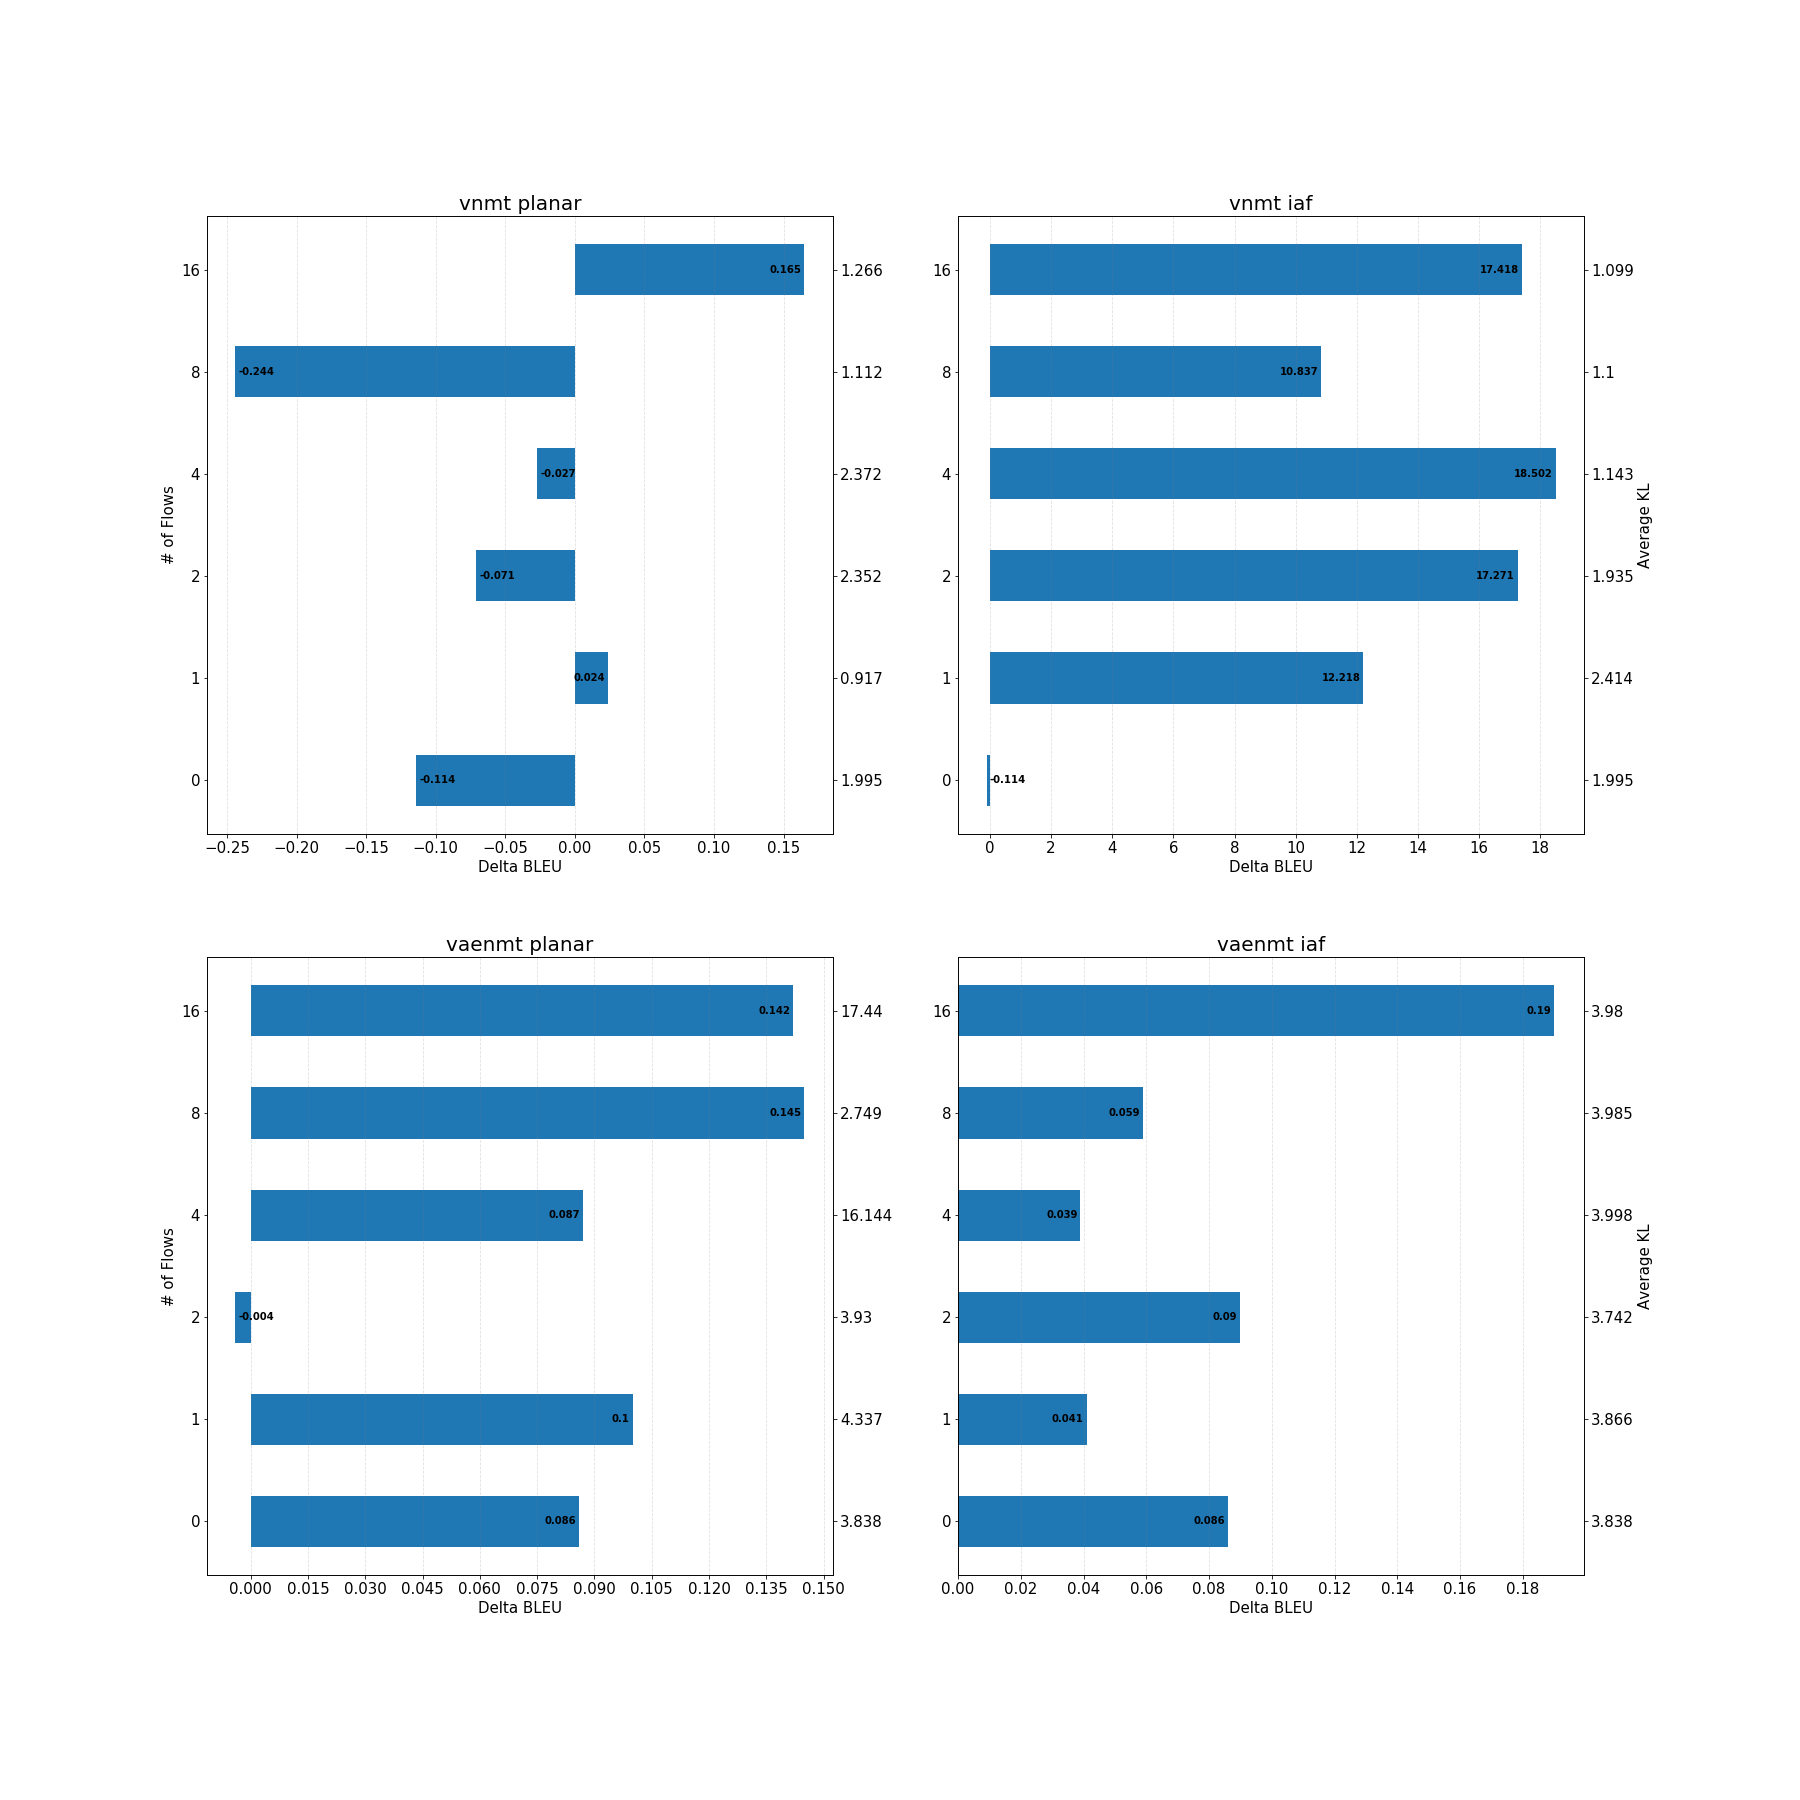
\includegraphics[width=\linewidth]{diff-z-256-horizontalbarplt.png}
	\caption{The drop in performance when we set the value of the latent variable of Z to 0 during evaluation for latent dimensions set to 256. Bars are $BLEU_{Z=\mu} - BLEU_{Z=0}$. KL divergence of model is included on right axis, number of flows on left axis.}
	\label{fig:barperfdrop}
\end{figure}

\section{Language Modelling Performance}

Hypothesis: Including normalizing flows improve the performance of the language model learned as part of the generative machine translation system. [This is related to a SPECIFIC model and is not applicable to the discriminative version of this stuff...just want to make sure that's clear]
As previously discussed in chapter 3, the generative machine translation system is trained with a language model component as part of the optimization process. In this section, we look at how the performance of this component is affected by the inclusion of normalizing flows by evaluating the performance of the learned language model during the training procedure. We measure the BLEU score and perplexity  [ are there other metrics I should consider?] for the generated source side sentences in our GNMT model. Note that the -ELBO in [Fig of ELBO] is already reported as this module is learned along with the translation system.

for Language model:
Intrinsic metric: generate sequence that is expected: Lower the better (evaluating itself against...itself? you can evaluate. Use perplexity => method of identifying how close the model will predict a given sequence. How close to the language model it was trained on. 

perplexity is sitll for the language model performance

Extrinsic evaluation: Put your language model into something else. e.g. plug into MT system, does it help machine translation?
How do we know if it helped or not? did bleu score go up or not? 
does the effect adding the language model vs adding flows
4 settings: LM + flows, LM + w/o flows, w/o LM + flows, w/o Lm model + w/o flows


extrinstic
\section{Importance of Attention}

Hypothesis:  Although performance will likely drop from the exclusion of attention in the translation system, we hypothesize that if the latent variable is adding additional information to the system, it wuold still outperform a vanilla RNN model without attention and that normalizing flows will further improve on this performance gain.

In much previous work that has included latent variables in the translation system they build on the system from \cite{bahndanau et. al.} . This model, as previously discussed, includes an attention mechanism that is fed as input to the decoder to provide contextual information during translation. As such, attention can be viewed as a confounding factor when adding additional inputs to the RNN via the latent variable. If anything, a more natural choice is to make the attention mechanism itself a random variable (pretty sure people have done this too btw....) instead of creating an additional latent variable that is conditioned on the same information. To better understand a latent variable as input for informing the decoding process, we remove attention and compare to a seq2seq model without attention or latent variables. In this setting, we add the latent variable as an additional input to the generator network (MLP that produces word probabilities) like the attention mechanism to see if this fixed global variable is useful in of itself. We then add normalizing flows on top of this to see if the learned distribution offers any further performance gains. We use the same settings as our translation experiments, where the only difference is without attention.

We measure ELBO, bleu, NLL again.
% #make sure code is clean

%\section{Out of Domain Translation}

%We considered different data sets to do this..

\section{Understanding Latent Variable}

considerations:
\begin{enumerate}
	\item set Z = 0 vector
	\item set Z ~ N(0, 1) vector
	\item set Z swapped with nearest neighbors??
	\item Visualize latent variables from transformation
\end{enumerate}